\documentclass[12pt,a4paper]{article}

\usepackage[T1]{fontenc}
\usepackage[utf8]{inputenc}
\usepackage{lmodern}
\usepackage{graphicx}
\usepackage{float}
\usepackage{geometry}
\usepackage{listings}
\usepackage{xcolor}
\usepackage{fancyhdr}
\usepackage{amsmath}
\usepackage{amssymb}
\usepackage{booktabs}
\usepackage{caption}
\usepackage{needspace}
\usepackage{array}
\usepackage{enumitem}
\usepackage{tikz}
\usepackage[section]{placeins}
\usepackage{tocloft}
\setlength{\cftbeforesecskip}{3pt}
\usepackage[hidelinks]{hyperref}
\usepackage{xurl}
\newcommand{\file}[1]{\nolinkurl{#1}}
\usetikzlibrary{arrows.meta,positioning}

\AddToHook{cmd/subsection/before}{\Needspace{8\baselineskip}}
% every section (the six phases, references and each appendix) starts on a new page
\AddToHook{cmd/section/before}{\clearpage}

\geometry{margin=1in}
\captionsetup{font=small,labelfont=bf}
\setlength{\textfloatsep}{14pt}
\setlength{\emergencystretch}{2em}
\setlength{\parskip}{5pt}
\setlength{\parindent}{0pt}
\setlist{itemsep=2pt,topsep=3pt}
\widowpenalty=10000 \clubpenalty=10000 \displaywidowpenalty=10000

\graphicspath{{../../figures/}{../eda/}{images/}}

\definecolor{navy}{HTML}{1B2A4A}
\definecolor{medtech}{HTML}{1A8FA8}
\newcolumntype{L}[1]{>{\raggedright\arraybackslash}p{#1}}
\newcommand{\var}[1]{\texttt{\detokenize{#1}}}

% ---------- interpretation block (same style as the phase reports) ----------
\newenvironment{interp}{\par\smallskip\noindent\begin{minipage}{\linewidth}\setlength{\parskip}{5pt}\textbf{\color{navy}Interpretation.}\ }{\end{minipage}\par\medskip}
% a block of text that is never split across two pages
\newenvironment{keep}{\par\noindent\begin{minipage}{\linewidth}\setlength{\parskip}{5pt}}{\end{minipage}\par\medskip}
\renewcommand{\topfraction}{0.9}\renewcommand{\bottomfraction}{0.8}\renewcommand{\textfraction}{0.07}\renewcommand{\floatpagefraction}{0.75}\setcounter{topnumber}{3}\setcounter{totalnumber}{5}

% ---------- parts to be completed by Yassine Mtibaa (CICIoT2023 phase 5) ----------
\newcommand{\tofill}[1]{\textcolor{red}{\textbf{[to fill: #1]}}}
\newcommand{\pending}[1]{%
\par\smallskip\noindent\fcolorbox{red!70!black}{red!3}{\parbox{\dimexpr\linewidth-2\fboxsep-2\fboxrule}{%
\textbf{\color{red!70!black}To be completed (Yassine Mtibaa, notebook \texttt{08\_features\_iot23}).} #1}}\par\smallskip}

% Figure that appears automatically once the file exists; otherwise a framed placeholder.
\newcommand{\labimage}[3][0.82\linewidth]{%
\begin{figure}[!htbp]
\centering
\IfFileExists{../../figures/#2}{%
    \includegraphics[width=#1,height=.42\textheight,keepaspectratio]{#2}%
}{%
    \fbox{\parbox[c][4.2cm][c]{0.8\linewidth}{\centering
    \textbf{FIGURE PLACEHOLDER}\\[0.3cm]
    Created when \texttt{08\_features\_iot23} is run:\\
    \texttt{\detokenize{figures/#2}}}}%
}
\caption{#3}\label{fig:#2}
\end{figure}
}

\newcommand{\fig}[3][0.9\linewidth]{%
\begin{figure}[!htbp]\centering
\includegraphics[width=#1,height=.45\textheight,keepaspectratio]{#2}
\caption{#3}\label{fig:#2}
\end{figure}}

\lstdefinestyle{mystyle}{
    basicstyle=\ttfamily\footnotesize, breaklines=true, columns=fullflexible, keepspaces=true,
    showstringspaces=false, xleftmargin=1.5em, numbers=left, numberstyle=\tiny,
    keywordstyle=\color{blue}, commentstyle=\color{green!50!black}, stringstyle=\color{red}}
\lstset{style=mystyle}

\setlength{\headheight}{15pt}
\pagestyle{fancy}
\fancyhf{}
\fancyhead[L]{CS434 - Data Science}
\fancyhead[R]{Cross-Network Intrusion Analysis}
\fancyfoot[C]{\thepage}

\tikzset{
  pstep/.style={draw, rounded corners, fill=medtech!10, minimum width=2.6cm, minimum height=1.1cm,
               align=center, font=\footnotesize},
  data/.style={draw, fill=orange!12, minimum width=2.6cm, minimum height=1.1cm, align=center, font=\footnotesize},
  flow/.style={-{Stealth[length=2.5mm]}, thick}
}

\begin{document}

% =========================================================
% TITLE PAGE
% =========================================================
\begin{titlepage}
\centering
\IfFileExists{images/MEDTECH-LOGO.png}{%
    
\includegraphics[width=7cm]{images/MEDTECH-LOGO.png}\\
}{\vspace*{1cm}}

\vspace{0.5cm}
{\Large \textbf{Mediterranean Institute of Technology}}\\[0.5cm]
{\large Computer System Engineering Program}\\

\vspace{2cm}
{\LARGE \textbf{Data Science Project Report}}\\[0.3cm]
{\large Course Code: CS434 -- Data Science}\\[0.6cm]
{\Large \textbf{Cross-Network Intrusion Analysis}}\\[0.2cm]
{\large Detecting Cyberattacks Across Five Network Environments with CRISP-DM}\\

\vspace{2cm}
{\Large \textbf{Submitted By:}}\\[0.2cm]
{\large Ahmed Hamouda}\\[0.1cm]
{\large Cyrine Chabbar}\\[0.1cm]
{\large Yassine Mtibaa}\\

\vspace{1.2cm}
{\Large \textbf{Professor:}}\\[0.2cm]
{\large Dorra Louati}\\[0.6cm]
{\Large \textbf{Lab Instructor:}}\\[0.2cm]
{\large Hamza Mouharrar}\\

\vfill
{\large \textbf{Date:} October 2026}
\end{titlepage}

% =========================================================
% ABSTRACT AND CONTENTS
% =========================================================
\section*{Abstract}
\addcontentsline{toc}{section}{Abstract}

Machine-learning intrusion detection systems are usually built and tested on a single network, so their reliability
on another network is unknown. This project follows the CRISP-DM process, from business understanding to feature
engineering, to prepare and analyse traffic from \textbf{five network environments}. The data are four NetFlow v3
datasets (UNSW-NB15, CSE-CIC-IDS2018, ToN-IoT, BoT-IoT) and CICIoT2023, mapped to one shared taxonomy of 9 attack
families.

\textbf{Preparing the data.} A systematic quality check found mislabelled traffic, columns broken by divisions by
zero, and duplicated captures. After the cleaning, the four NetFlow datasets were merged into one table of
\textbf{17,551,848 distinct behaviours representing 63,012,224 flows}. CICIoT2023 was kept separate (20,701,050 clean
packet windows), because a row there measures something different.

\textbf{What the analysis shows.}
\begin{enumerate}
  \item No traffic variable is normally distributed, so non-parametric tests are used.
  \item Attack and normal traffic differ strongly inside each network, but \emph{in opposite directions} in different
        networks: attacks are smaller than normal traffic in UNSW-NB15 and larger in ToN-IoT.
  \item The same attack family does not produce the same traffic in different networks (Kolmogorov--Smirnov distance
        up to 0.99), nor in a different dataset.
\end{enumerate}

\textbf{Feature engineering} produced a justified set of \textbf{59 features} for the NetFlow data, with every
identifier of the network or the lab removed, and \textbf{31 features} for CICIoT2023. These results point to a
clear expectation for the next step: a detector trained on some networks will lose accuracy on a new network, and
the modelling plan proposed at the end is designed to measure that loss.

\newpage
{\setlength{\parskip}{0pt}\small\tableofcontents}
\newpage

% =========================================================
% 1 BUSINESS UNDERSTANDING
% =========================================================
\section{Business Understanding}

\subsection{Project context}
Every organisation connected to the internet is a target: its network is probed by scans, flooded by
denial-of-service attacks, attacked with password guessing, and infected by malware that turns its devices into bots.
\textbf{Network Intrusion Detection Systems (NIDS)} monitor the traffic and raise an alert when it looks malicious.
Security teams face two costly failures: \textbf{missed attacks}, and \textbf{false alarms} that waste analysts' time
until real alerts are ignored.

Modern NIDS increasingly use machine learning, learning what attacks look like from labelled traffic. But organisations
run very different networks (offices, industrial IoT, smart devices), and a detector trained on one kind of network
often performs much worse on another. An organisation usually cannot collect and label its own attack data before
deploying a detector.

\subsection{Problem statement}
\begin{quote}
Organisations need an intrusion detection approach that recognises cyberattacks accurately, tells the security team
\textbf{what kind} of attack is happening, and stays reliable on a \textbf{different type of network} from the one it
was trained on.
\end{quote}
As a data science problem:
\begin{enumerate}
  \item integrate traffic recorded on five different networks into consistent, analysis-ready data;
  \item organise all attack types into one shared taxonomy;
  \item analyse which traffic characteristics reveal each attack family, and whether they hold from one network to
        another;
  \item prepare the features for a future classifier.
\end{enumerate}

\subsection{Research questions}
\textbf{Main question:} \emph{How can traffic collected from different network environments be used to detect
cyberattacks and identify their type reliably, including on networks the detection model has never seen?} It is broken into three sub-questions (Table~\ref{tab:sq}).

\begin{table}[H]\centering\small
\caption{Sub-questions. SQ1 identifies \emph{what} reveals an attack, SQ2 tests \emph{whether} it transfers between
networks, SQ3 asks \emph{how well} a model could use it.}\label{tab:sq}
\begin{tabular}{lL{13.2cm}}
\toprule
\textbf{SQ1} & Which traffic characteristics best distinguish normal traffic from attack traffic, and how do they differ
across attack families? \\
\textbf{SQ2} & How consistent is the traffic behaviour of the same attack type across different network environments? \\
\textbf{SQ3} & How accurately could a model detect attacks and identify their family, and how much would its performance
change on a network it was not trained on? \\
\bottomrule
\end{tabular}
\end{table}

\subsection{Success criteria}
The project is successful if:
\begin{enumerate}
  \item \textbf{every sub-question is answered with evidence}: statistical tests, effect sizes and figures, not
        assumptions;
  \item \textbf{the key indicators of each attack family are identified}: we can explain what gives each type of
        attack away;
  \item \textbf{the data are model-ready and free of leakage}: a justified final feature set with no column that
        identifies the network, the machine or the moment;
  \item \textbf{the work is understandable and reproducible}: every decision is documented, and anyone can rebuild
        the results from the repository.
\end{enumerate}
Model training is outside the scope of this project; SQ3 is answered as an evidence-based expectation and a modelling
plan (Section~6).

% =========================================================
% 2 DATA UNDERSTANDING
% =========================================================
\section{Data Understanding}

\subsection{Data sources and provenance}
Five public datasets cover five network environments. The four NetFlow v3 datasets were re-extracted by the University
of Queensland from the original packet captures with the same tool (nProbe) into the same 53 features, so a column
means exactly the same thing in all four files \cite{luay2025,sarhan2022}. CICIoT2023 was recorded on 105 real IoT
devices with a different feature extractor \cite{ciciot2023}. Table~\ref{tab:datasets} summarises the five datasets.

\begin{table}[!htbp]\centering\small
\caption{The five datasets. Flows and attack shares are counted in the loaded files.}\label{tab:datasets}
\footnotesize\setlength{\tabcolsep}{4pt}
\begin{tabular}{L{4.1cm}L{2.7cm}rrrL{1.9cm}}
\toprule
Dataset & Network environment & Rows & Attack \% & Attack labels & Owner \\
\midrule
NF-UNSW-NB15-v3 \cite{unsw} & Mixed lab network & 2,365,424 & 5.4 & 9 & A.~Hamouda \\
NF-CSE-CIC-IDS2018-v3 \cite{cic2018} & Enterprise / office & 20,115,529 & 12.9 & 14 & A.~Hamouda \\
NF-ToN-IoT-v3 \cite{ton} & IoT / industrial & 27,520,260 & 39.0 & 9 & C.~Chabbar \\
NF-BoT-IoT-v3 \cite{bot} & IoT botnet & 16,933,808 & 99.7 & 4 & C.~Chabbar \\
CICIoT2023 \cite{ciciot2023} & 105 real IoT devices & 45,019,243$^{*}$ & 97.7 & 33 & Y.~Mtibaa \\
\bottomrule
\end{tabular}

\smallskip{\footnotesize $^{*}$ packet windows, not flows.}
\end{table}

\subsection{Dimensions and structure}
\begin{itemize}
  \item \textbf{NetFlow v3:} each row is \textbf{one flow} (a connection from its first to its last packet), with 53
        features plus \var{Label} (0/1) and \var{Attack} (class name). The loaded row counts match the official
        numbers except BoT-IoT. Its page states 16,993,808 rows, but the file has 16,933,808, which is also the sum of
        its own Benign and attack counts: a typo on the official page.
  \item \textbf{CICIoT2023:} each row is \textbf{one window of up to 100 packets}, described by 39 statistics (shares
        of packets per protocol and flag, packet-size statistics, rate) plus \var{Label}. We used the newer
        \texttt{MERGED\_CSV} release (63 files, 9.3\,GB). It differs from the 2023 documentation: 45,019,243 rows
        instead of 46.7 million, and 8 columns removed or renamed.
\end{itemize}

\subsection{Variables, data types and units}
Table~\ref{tab:vars} groups the NetFlow variables by role, with their type and unit.
\begin{table}[!htbp]\centering\small
\caption{NetFlow v3 variables by group. The full dictionary of the 53 features (meaning, unit, type and what happened
to each) is in Appendix~B.}\label{tab:vars}
\begin{tabular}{L{2.7cm}L{6.1cm}L{2.3cm}L{2.5cm}}
\toprule
Group & Example columns & Type & Unit \\
\midrule
Identifiers & \var{IPV4_SRC_ADDR}, \var{L4_SRC_PORT}, \var{DNS_QUERY_ID} & text / code & -- \\
Protocol / service & \var{PROTOCOL}, \var{L4_DST_PORT}, \var{L7_PROTO} & code & -- \\
Volume & \var{IN_BYTES}, \var{OUT_BYTES}, \var{IN_PKTS}, \var{OUT_PKTS} & integer & bytes, packets \\
Packet sizes & \var{LONGEST_FLOW_PKT}, \var{NUM_PKTS_UP_TO_128_BYTES} & integer & bytes, packets \\
Time & \var{FLOW_DURATION_MILLISECONDS}, \var{SRC_TO_DST_IAT_AVG} & integer & ms \\
Timestamps & \var{FLOW_START_MILLISECONDS} & integer & ms since 1970 \\
TCP behaviour & \var{CLIENT_TCP_FLAGS} (bitmask), \var{TCP_WIN_MAX_IN} & code / integer & --, bytes \\
Labels & \var{Label}, \var{Attack} & integer / text & -- \\
\bottomrule
\end{tabular}
\end{table}

\textbf{Key variables.} The volume, packet-size and timing columns describe \emph{what the traffic does}; the
destination port, protocol and TCP flags describe \emph{how}. For CICIoT2023 the key variables are \var{Rate}
(packets/s), the packet-size statistics (\var{AVG}, \var{Std}, \var{Max}), the protocol and flag shares, \var{IAT} and
\var{Header_Length}.

\subsection{A shared attack taxonomy}
The five datasets name their attacks differently (54 labels, often with different spellings), so every label was
mapped to one of \textbf{9 attack families}: Denial of service, Reconnaissance, Credential attacks, Web and injection,
Malware and botnets, Exploitation and intrusion, Interception and spoofing, Fuzzing and crypto, Data theft. The mapping
is fixed in the shared code (\texttt{src/config.py}), so every dataset uses the same families.

\fig[0.72\linewidth]{NetFlow_eda_families.png}{Share of each family in the merged NetFlow data, counted in distinct
behaviours and in flows (after cleaning).}

\fig[0.82\linewidth]{IoT23_class_distribution.png}{CICIoT2023: number of rows per attack label before sampling (log
scale). The largest label is 5,764 times the smallest.}

\begin{interp}
Both data sources are strongly imbalanced, but in different ways (Figures~\ref{fig:NetFlow_eda_families.png} and~\ref{fig:IoT23_class_distribution.png}). In NetFlow, Benign dominates the distinct
behaviours (67\%), while Denial of service dominates the flows (33\%) because a flood repeats the same flow millions of
times. CICIoT2023 is 97.7\% attacks, mostly floods. Not every family exists in every network: only Benign and Denial
of service are present in all four NetFlow networks, which limits the comparisons across networks (SQ2).
\end{interp}

\subsection{Initial quality issues and limitations}
Each dataset went through the same checks, following the course lab: structure, missing and infinite values, data
types, outliers (IQR, z-score, box plots), consistency (duplicates, identifiers, logical rules) and class distribution.
For NetFlow, every problem was documented with evidence in a dedicated report, split into problems solved before the
merge (codes U, C, T, B) and after it (M), and findings kept on purpose (K). Table~\ref{tab:issues} lists the most important ones.

\begin{table}[!htbp]\centering\small
\caption{The most important quality issues found (phase 2, diagnosis only).}\label{tab:issues}
\begin{tabular}{L{4.4cm}L{6.2cm}L{3.8cm}}
\toprule
Issue & Evidence & Dataset \\
\midrule
NaN / infinite rates & bytes $\div$ 0 on 0-ms flows: 387,350 NaN + 1,716,860 inf (65\% of Benign) & BoT-IoT, UNSW \\
Two codes in one number & \var{L7_PROTO} = \texttt{5.239} (DNS carrying another protocol) & UNSW, BoT-IoT \\
Duplicated captures & 628,474 rows (CIC18), 1,816,137 (ToN); 51\% of CICIoT2023 & all \\
Mislabelled traffic & ``DoS SlowHTTPTest'' flows are refused FTP connections (105,550) & CIC-2018 \\
Labels on normal traffic & 150,600 attack flows identical to Benign flows of the same machines & CIC-2018 \\
Web attacks on DNS traffic & 1,261,353 ``XSS'' / ``injection'' flows to port 53 & ToN-IoT \\
Same flow, two labels & 880 rows (NetFlow); 13.3 M rows, mostly DoS vs DDoS (CICIoT2023) & CIC-2018, CICIoT2023 \\
Identifiers that reveal the label & IP addresses, timestamps, TTL, TCP window & all \\
Documentation errors & BoT-IoT row count; release differs from paper (CICIoT2023) & BoT-IoT, CICIoT2023 \\
\bottomrule
\end{tabular}
\end{table}



% =========================================================
% 3 DATA PREPROCESSING
% =========================================================
\section{Data Preprocessing}

\subsection{Principles}
\begin{itemize}
  \item \textbf{One shared code base.} Every member uses the same functions (\texttt{src/config.py}: cleaning, label
        mapping, validation), so differences between networks reflect the traffic, not the preprocessing.
  \item \textbf{Decide first, then apply.} Every treatment was proposed in phase 2, approved by the team, and recorded
        in the decision log before being applied in phase 3.
  \item \textbf{Evidence before and after.} Each cleaning notebook reports row counts and checks after every step
        (\texttt{tables/*\_quality.csv}).
\end{itemize}

\begin{figure}[!htbp]\centering
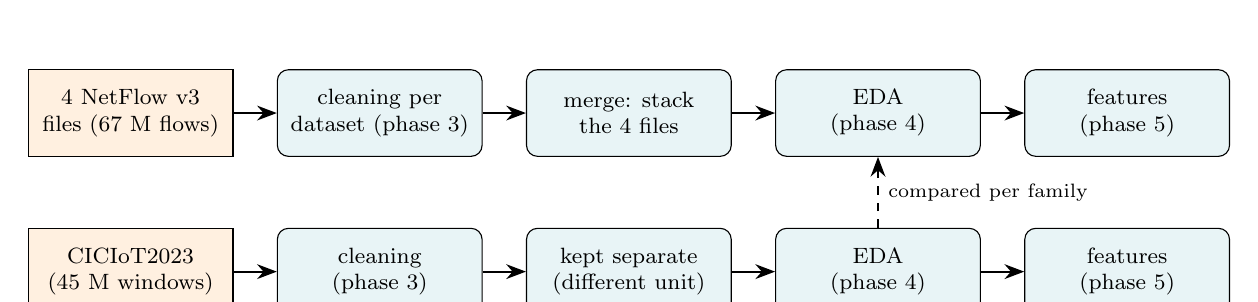
\begin{tikzpicture}[node distance=0.55cm and 0.55cm]
\node[data] (raw) {4 NetFlow v3\\files (67 M flows)};
\node[pstep, right=of raw] (clean) {cleaning per\\dataset (phase 3)};
\node[pstep, right=of clean] (merge) {merge: stack\\the 4 files};
\node[pstep, right=of merge] (eda) {EDA\\(phase 4)};
\node[pstep, right=of eda] (fe) {features\\(phase 5)};
\node[data, below=0.9cm of raw] (iraw) {CICIoT2023\\(45 M windows)};
\node[pstep, right=of iraw] (iclean) {cleaning\\(phase 3)};
\node[pstep, right=of iclean] (isep) {kept separate\\(different unit)};
\node[pstep, right=of isep] (ieda) {EDA\\(phase 4)};
\node[pstep, right=of ieda] (ife) {features\\(phase 5)};
\draw[flow] (raw) -- (clean); \draw[flow] (clean) -- (merge); \draw[flow] (merge) -- (eda); \draw[flow] (eda) -- (fe);
\draw[flow] (iraw) -- (iclean); \draw[flow] (iclean) -- (isep); \draw[flow] (isep) -- (ieda); \draw[flow] (ieda) -- (ife);
\draw[flow, dashed] (ieda) -- node[right, font=\scriptsize]{compared per family} (eda);
\end{tikzpicture}
\caption{The data pipeline. NetFlow and CICIoT2023 are processed with the same steps; they are compared at the level of
attack families, never merged.}
\end{figure}

\subsection{Cleaning each NetFlow dataset}
Each NetFlow dataset has its own cleaning notebook, which applies only that dataset's approved decisions, in this
order:
\begin{enumerate}
  \item \textbf{Fix broken columns.} The two bytes-per-second columns are dropped (U2, B2, C3, T3). They are NaN or
        infinite on every 0-ms flow; deleting those rows instead would have removed 65\% of BoT-IoT's Benign traffic.
        \var{L7_PROTO} is split into two integer codes, \var{L7_MAIN} and \var{L7_SUB} (U3, B3).
  \item \textbf{Remove exact duplicate rows} (U4, C4, T4).
  \item \textbf{Remove mislabelled traffic} (C5--C7, T5). Flows that carry two labels, SlowHTTPTest flows that are
        refused FTP connections, attack labels on flows identical to Benign traffic of the same machines, and web
        attacks labelled on DNS traffic. Relabelling them as Benign was considered and rejected, because it would
        invent labels.
  \item \textbf{One row per distinct behaviour.} Identical flows (same behaviour, ignoring IPs, ports and timestamps)
        are merged into one row with a \var{count} column. This replaces the planned cap of 200,000 flows per label,
        which would have kept only 15--40\% of the distinct attack behaviours of the large classes.
  \item \textbf{Standard cleaning and label mapping:} identifiers dropped, labels mapped to the taxonomy,
        \var{Label} dropped (identical to \var{is_attack}).
  \item \textbf{Validation:} \var{validate()} reports 0 violations, and there are no NaN or infinite values.
\end{enumerate}

\textbf{Outliers.} Extreme values (huge floods, long connections, packets above 1,514 bytes) were \textbf{kept}: in
this data the outliers are the attacks. Only impossible values were changed (DNS TTL above $2^{31}-1$, set to 0 as
RFC 2181 prescribes). Table~\ref{tab:cleaning} shows the effect of the cleaning on each dataset.

\begin{table}[!htbp]\centering\small
\caption{Effect of the cleaning on each NetFlow dataset.}\label{tab:cleaning}
\begin{tabular}{lrrrL{5.4cm}}
\toprule
Dataset & Raw flows & Clean rows & Flows kept & Main removals \\
\midrule
UNSW & 2,365,424 & 1,405,100 & 2,350,609 & 14,815 duplicates \\
CIC-2018 & 20,115,529 & 8,945,792 & 19,285,037 & 628,474 duplicates; 880 + 105,580 + 95,558 mislabelled \\
ToN-IoT & 27,520,260 & 5,637,642 & 24,442,770 & 1,816,137 duplicates; 1,261,353 web attacks on DNS \\
BoT-IoT & 16,933,808 & 1,563,315 & 16,933,808 & none (only collapsed into behaviours) \\
\bottomrule
\end{tabular}
\end{table}

\subsection{Integration: merging the four NetFlow datasets}
The four cleaned files have the same columns, so they are \textbf{stacked} (\var{pd.concat}), not joined: they
contain different flows from different networks and share no key. A column \var{source_dataset} records the
network; like \var{count}, it is never a model feature. Some decisions need all four datasets together, so they are
applied once on the merged table (Table~\ref{tab:merge}).

\begin{table}[!htbp]\centering\small
\caption{Decisions applied after the merge.}\label{tab:merge}
\begin{tabular}{lL{6.6cm}L{6.2cm}}
\toprule
Code & Decision & Effect \\
\midrule
M1, M2 & codes $\rightarrow$ categories; timestamps $\rightarrow$ dates (never features) & 10 code columns, 2 timestamps \\
M6 & ICMP fields set to 0 outside ICMP flows & 2,879,966 rows corrected \\
M7, M8 & drop columns that copy others (\var{MIN/MAX_IP_PKT_LEN}, \var{TCP_FLAGS}, \var{ICMP_IPV4_TYPE}) & 4 columns removed, no information lost \\
M9 & invalid DNS TTL $\rightarrow$ 0 & 14 rows; 1 row merged into an identical one \\
M11 & flag behaviours that have a different family in another dataset & 38,453 rows flagged, none removed \\
\bottomrule
\end{tabular}
\end{table}

\textbf{Result:} \texttt{netflow\_merged.parquet}, \textbf{17,551,848 rows representing 63,012,224 flows}, 54 columns,
0 missing values, 0 validation violations.

\subsection{Cleaning CICIoT2023, and why it stays separate}
\begin{itemize}
  \item \textbf{Treatments.} Impossible values were removed: 7 truncated lines, 991 windows with an infinite
        \var{Rate} (0-second windows, which have no meaningful rate, so nothing was imputed) and 2 negative \var{IAT}
        values. Exact duplicates were removed per file and again after combining the 63 files, and labels were mapped
        to the taxonomy. At most 200,000 rows were kept per label. Windows whose features also appear under another
        label (mostly DoS vs DDoS) were \textbf{kept and flagged} (\var{conflicting_features}) for the EDA.
  \item \textbf{Result:} 45,019,243 $\rightarrow$ 20,701,050 clean windows (24.3 M duplicates removed)
        $\rightarrow$ 4,420,714 sampled rows; 0 missing, 0 infinite.
  \item \textbf{Why not merged with NetFlow.} A CICIoT2023 row is a window of up to 100 packets that can mix several
        connections; a NetFlow row is one connection. The 39 window statistics (shares of packets per flag) are not
        the same measurements as the 53 flow features (bitmasks per flow). Stacking them would put incompatible
        values in the same column. The datasets are compared at the level of attack families instead (Section~4.7).
\end{itemize}

\fig[0.72\linewidth]{IoT23_rows_per_family_phase3.png}{CICIoT2023: rows per family after cleaning and sampling.}

\subsection{Preventing data leakage}
Columns that reveal the answer are \textbf{never features}: IP addresses (they identify the attacker machine),
timestamps (they reveal the lab's attack schedule), TTL and TCP window (set by each lab machine's operating system),
random identifiers, \var{source_dataset} and \var{count}. Mislabelled flows are removed rather than relabelled, so no
label is invented.

% =========================================================
% 4 EXPLORATORY DATA ANALYSIS
% =========================================================
\section{Exploratory Data Analysis}

The analysis follows the course lab (Lab 4). For NetFlow, every statistic is computed on the \textbf{17.5 million
distinct behaviours}: identical copies of a flow are not independent observations and would let the floods dominate.
Box plots, correlation and the Kolmogorov--Smirnov test use a stratified sample of up to 10,000 behaviours per
network $\times$ family (187,418 rows), so every family is represented. For CICIoT2023, the analysis uses the sampled
cleaned data (4.4 M windows).

\subsection{Descriptive statistics}
\begin{table}[!htbp]\centering\small
\caption{Merged NetFlow: summary statistics of the key variables (all 17.5 M behaviours).}\label{tab:summary}
\begin{tabular}{lrrrrr}
\toprule
Variable & Mean & Median & IQR & Skewness & Max \\
\midrule
\var{IN_BYTES} & 3,725 & 701 & 1,459 & 357.2 & 189,027,266 \\
\var{OUT_BYTES} & 11,338 & 940 & 2,112 & 194.5 & 196,978,660 \\
\var{IN_PKTS} & 32.9 & 6 & 7 & 179.4 & 1,220,131 \\
\var{FLOW_DURATION_MILLISECONDS} & 14,549 & 755 & 4,010 & 2.4 & 120,999 \\
\bottomrule
\end{tabular}
\end{table}

\begin{interp}
Every variable is strongly \textbf{right-skewed} in both datasets (Table~\ref{tab:summary}): the mean is far above the median because a few
gigantic flows (up to 189\,MB) pull it up, and the skewness is far above 1. In CICIoT2023, \var{Rate} has a mean of
14,219 packets/s but a median of 5,258 (skewness 35.8), and \var{IAT} has a skewness of 1,821. The \textbf{median and
the IQR} therefore describe a typical flow better, and log scales are used in the plots. The NetFlow duration never
exceeds 121\,s because the exporter cuts longer connections.
\end{interp}

\begin{table}[!htbp]\centering\small
\caption{Merged NetFlow: median per family.}\label{tab:famdesc}
\begin{tabular}{lrrrr}
\toprule
Family & \var{IN_BYTES} & \var{OUT_BYTES} & \var{IN_PKTS} & Duration (ms) \\
\midrule
Benign & 1,135 & 1,572 & 8 & 1,325 \\
Denial of service & 528 & 1,136 & 6 & 10,812 \\
Reconnaissance & 44 & 40 & 1 & 23 \\
Credential attacks & 481 & 2,142 & 6 & 438 \\
Web and injection & 760 & 1,304 & 6 & 304 \\
Malware and botnets & 288 & 240 & 6 & 1,506 \\
Exploitation and intrusion & 822 & 555 & 10 & 800 \\
Interception and spoofing & 140 & 258 & 2 & 37 \\
Fuzzing and crypto & 812 & 336 & 10 & 708 \\
Data theft & 1,658 & 3,380 & 14 & 2,407 \\
\bottomrule
\end{tabular}
\end{table}

\begin{interp}
Each family has its own typical flow (Table~\ref{tab:famdesc}):
\begin{itemize}
  \item \textbf{Reconnaissance} is a single probe packet (44 bytes, 1 packet);
  \item \textbf{Denial of service} holds connections open (median 10.8\,s);
  \item \textbf{Data theft} moves the most data.
\end{itemize}
In CICIoT2023 the families are just as distinct:
\begin{itemize}
  \item \textbf{DoS} windows are minimum-size packets (60\,B) at about 12,000 packets/s;
  \item \textbf{Mirai} floods use large, uniform packets (573\,B);
  \item \textbf{Benign} traffic has large, variable packets at a low rate.
\end{itemize}
The traffic variables therefore carry information about the attack family (SQ1).
\end{interp}

\subsection{Distributions}
\fig[0.98\linewidth]{NetFlow_eda_histograms.png}{Merged NetFlow: key variables on a $\log_{10}(1+x)$ scale (all
behaviours).}

\fig[0.98\linewidth]{NetFlow_eda_boxplots_by_family.png}{Merged NetFlow: bytes sent and flow duration by family
(stratified sample, log scale).}

\fig[0.98\linewidth]{IoT23_eda_distributions_by_family.png}{CICIoT2023: distributions of the key variables by family
(log scale).}

\begin{interp}
None of the variables has a bell shape (Figures~\ref{fig:NetFlow_eda_histograms.png}--\ref{fig:IoT23_eda_distributions_by_family.png}); the distributions show tall spikes at technical values:
\begin{itemize}
  \item no answer (\var{OUT_BYTES} = 0 for 8.8\% of NetFlow behaviours);
  \item one-packet flows;
  \item the 120\,s exporter limit;
  \item 1,500-byte Ethernet frames.
\end{itemize}
The families are clearly shifted from each other, but \textbf{the Benign range covers almost all attack families}: no
single variable separates normal traffic from every attack, so a detector needs several variables together.
\end{interp}

\subsection{Correlation analysis}
\begin{figure}[!htbp]\centering
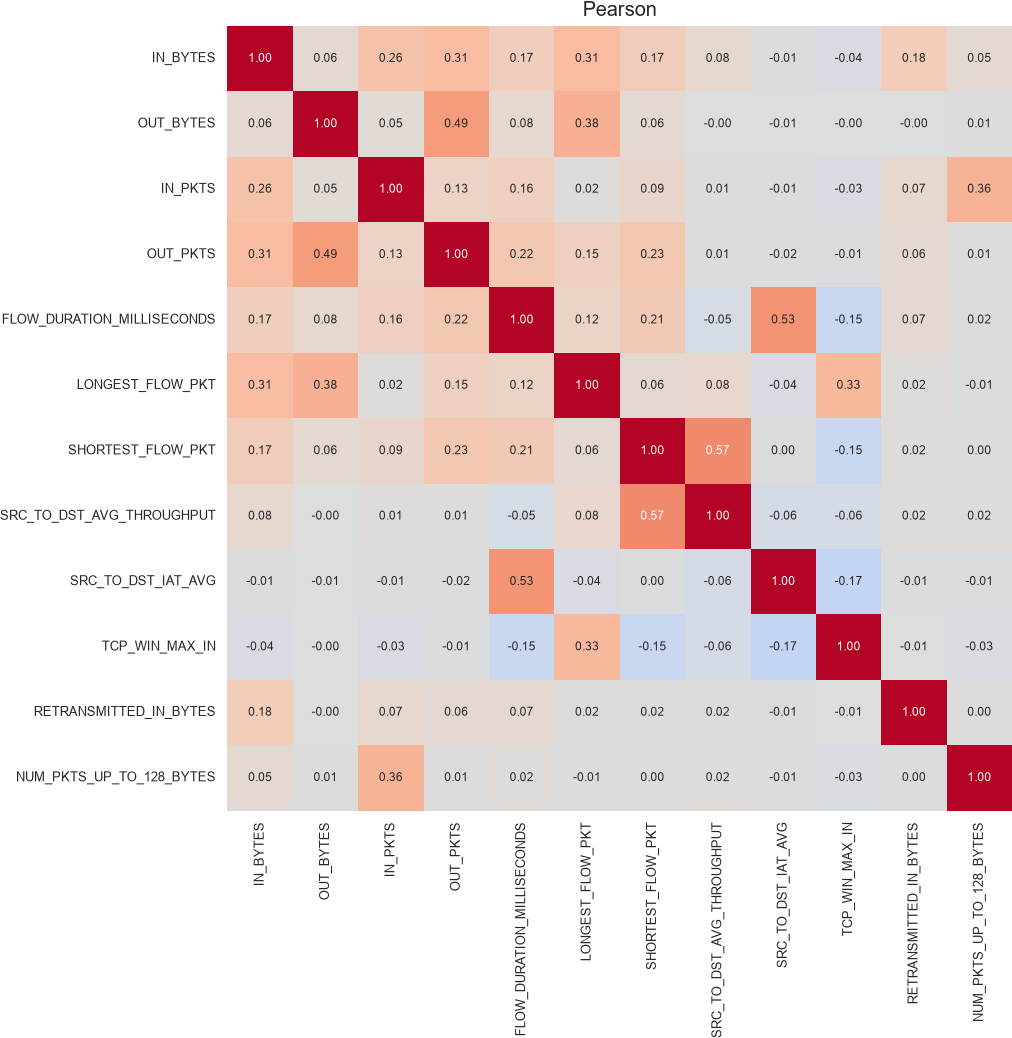
\includegraphics[width=0.48\linewidth]{corr_pearson.png}\hfill
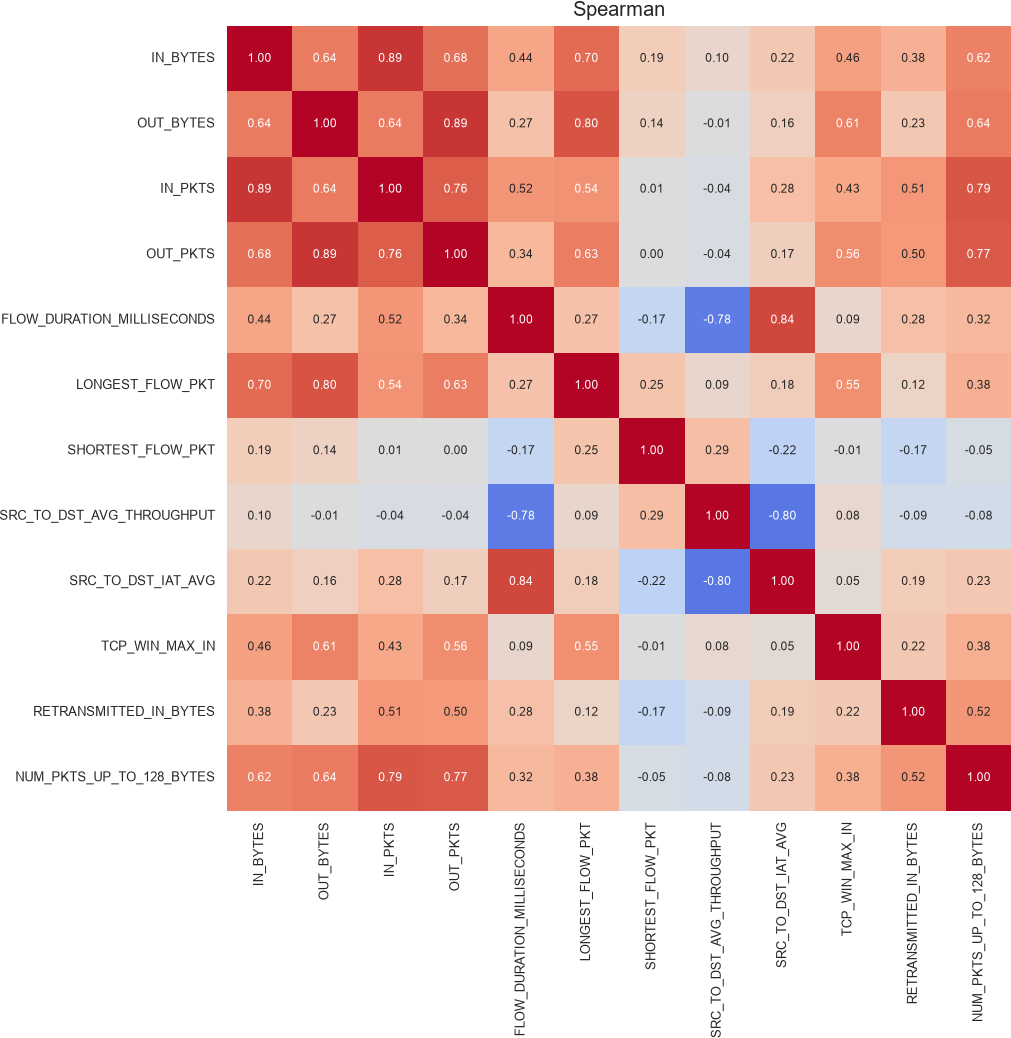
\includegraphics[width=0.48\linewidth]{corr_spearman.png}
\caption{Merged NetFlow: Pearson (left) and Spearman (right) correlation of 12 traffic features (stratified sample).}\label{fig:corr}
\end{figure}

\fig[0.66\linewidth]{IoT23_eda_correlation_heatmap.png}{CICIoT2023: Spearman correlation of the window features.}

\begin{interp}
Pearson finds almost no relationship in NetFlow, while Spearman finds strong ones (Figure~\ref{fig:corr}): for \var{IN_BYTES}--\var{IN_PKTS},
$r = 0.26$ but $\rho = 0.89$. Pearson measures straight lines and is dominated by a few gigantic flows; Spearman works
on ranks, so it is the right coefficient for these skewed data. In NetFlow, bytes and packets rise together
($\rho = 0.89$), and longer flows have longer gaps between packets ($\rho = 0.84$). CICIoT2023 has 12 pairs with
$|\rho| \geq 0.9$, several of them exact formulas:
\begin{itemize}
  \item \var{AVG} = \var{Tot_size};
  \item \var{Variance} = \var{Std}$^2$;
  \item \var{ARP} = 1 $-$ \var{IPv};
  \item \var{Rate} $\approx$ 1/\var{IAT} ($\rho = -0.995$).
\end{itemize}
Such redundant columns are removed in feature selection (Section~5).
\end{interp}

\subsection{Relationships between variables}
\fig[0.98\linewidth]{NetFlow_eda_benign_vs_attack.png}{Merged NetFlow: bytes and packets sent, Benign against attack,
in each network (stratified sample, log scale).}

\begin{table}[!htbp]\centering\small
\caption{Merged NetFlow: median of Benign against attack traffic in each network (all behaviours).}\label{tab:benatt}
\begin{tabular}{lrrrrrr}
\toprule
& \multicolumn{2}{c}{\var{IN_BYTES}} & \multicolumn{2}{c}{\var{IN_PKTS}} & \multicolumn{2}{c}{Duration (ms)} \\
\cmidrule(lr){2-3}\cmidrule(lr){4-5}\cmidrule(lr){6-7}
Network & Benign & Attack & Benign & Attack & Benign & Attack \\
\midrule
UNSW & 2,750 & 814 & 40 & 10 & 95 & 716 \\
CIC-2018 & 1,369 & 510 & 8 & 5 & 2,845 & 3,334 \\
ToN-IoT & 65 & 637 & 1 & 6 & 22 & 377 \\
BoT-IoT & 120 & 44 & 3 & 1 & 31 & 51 \\
\bottomrule
\end{tabular}
\end{table}

\begin{interp}
This is the central finding (Figure~\ref{fig:NetFlow_eda_benign_vs_attack.png} and Table~\ref{tab:benatt}): \textbf{the difference between Benign and attack traffic points in opposite directions in
different networks}. In UNSW-NB15, attacks are \emph{smaller} than normal traffic (814 vs 2,750 bytes). In ToN-IoT,
they are \emph{larger} (637 vs 65 bytes), because ToN-IoT's normal traffic consists mostly of tiny one-packet flows.
Normal traffic itself differs by a factor of 40 between networks. A rule such as ``attacks send more bytes'' holds in
one network and fails in another.
\end{interp}

\fig[0.72\linewidth]{NetFlow_eda_port_range_by_family.png}{Merged NetFlow: destination port range within each family
(\% of behaviours, all data).}

\fig[0.85\linewidth]{IoT23_eda_flag_fingerprints.png}{CICIoT2023: TCP-flag and protocol fingerprint of every attack
label (share of packets).}

\begin{interp}
The way traffic connects is strongly linked to the family (Figures~\ref{fig:NetFlow_eda_port_range_by_family.png} and~\ref{fig:IoT23_eda_flag_fingerprints.png}).
\begin{itemize}
  \item \textbf{NetFlow:} web, credential and denial-of-service traffic goes almost only to well-known ports
        (93--100\%), while reconnaissance goes 91\% to high ports, because a scan tries many ports.
  \item \textbf{CICIoT2023:} each flood has a fingerprint. SYN floods are about 100\% SYN, PSH-ACK floods 93\% PSH and
        ACK, ICMP floods 99\% ICMP, and Mirai floods use GRE. The low-volume attacks (reconnaissance, web,
        credential) look like normal traffic.
\end{itemize}
\end{interp}

\subsection{Normality and the choice of tests}
\fig[0.8\linewidth]{NetFlow_eda_normality_qq.png}{Merged NetFlow: Q-Q plots of \var{IN_BYTES} against the normal
distribution, raw (left) and $\log(1+x)$ (right).}

\fig[0.95\linewidth]{IoT23_eda_normality_qq.png}{CICIoT2023: histograms against the normal curve and Q-Q plots of the
key variables, raw and $\log(1+x)$.}

\begin{interp}
Shapiro--Wilk (on 5,000 values, its limit) and D'Agostino--Pearson reject normality (Figures~\ref{fig:NetFlow_eda_normality_qq.png} and~\ref{fig:IoT23_eda_normality_qq.png}) for \textbf{every variable, raw
and log-transformed, in both datasets} (all $p < 10^{-20}$), and also inside every family. The Q-Q plots confirm that
the departures are large, not a sample-size artefact. \textbf{Consequence:} the t-test and ANOVA, which assume normal
groups, are not suitable, so rank-based (non-parametric) tests are used. With millions of rows every p-value is close
to 0, so each test also reports an \textbf{effect size}, and conclusions rest on it. Several tests answer one
question, so p-values are Bonferroni-corrected.
\end{interp}

\subsection{Hypothesis tests}
\begin{keep}
\textbf{Test 1 (SQ1): Mann--Whitney U, NetFlow, attack vs Benign in each network.}\par
\begin{itemize}
  \item \textbf{H$_0$:} attack and Benign behaviours have the same distribution of the variable. \textbf{H$_1$:} they
        differ.
  \item \textbf{Assumptions checked and test chosen:} independent groups (one row per behaviour); normality rejected,
        so Mann--Whitney U instead of the two-sample t-test. All behaviours are used, which gives 16 tests.
  \item \textbf{Effect size:} rank-biserial $r = 2U/(n_1 n_2) - 1$; $r < 0$ means attacks are smaller. $|r| \geq 0.5$
        is a large effect.
\end{itemize}
\end{keep}

\begin{table}[!htbp]\centering\small
\caption{Mann--Whitney U: effect size $r$ of attack against Benign. All 16 tests reject H$_0$
(Bonferroni-corrected $p < 10^{-180}$).}\label{tab:mw}
\begin{tabular}{lrrrr}
\toprule
Variable & UNSW & CIC-2018 & ToN-IoT & BoT-IoT \\
\midrule
\var{IN_BYTES} & $-0.50$ & $-0.11$ & $+0.51$ & $-0.10$ \\
\var{OUT_BYTES} & $-0.73$ & $+0.04$ & $+0.69$ & $-0.13$ \\
\var{IN_PKTS} & $-0.62$ & $-0.11$ & $+0.59$ & $-0.22$ \\
\var{FLOW_DURATION_MILLISECONDS} & $+0.46$ & $-0.05$ & $+0.36$ & $+0.12$ \\
\bottomrule
\end{tabular}
\end{table}

\begin{interp}
\textbf{Decision ($\alpha = 0.05$):} reject H$_0$ in all 16 tests (Table~\ref{tab:mw}). The effects are large in UNSW (attacks
\emph{smaller}, $r$ down to $-0.73$; a random attack flow receives more data than a random Benign flow only 14\% of the
time) and in ToN-IoT (attacks \emph{larger}, $r$ up to $+0.69$), and small in CIC-2018 and BoT-IoT. \textbf{Answer to
SQ1:} attack traffic does differ from normal traffic, often strongly, but \textbf{which variable shows it and in which
direction depends on the network}.
\end{interp}

\begin{keep}
\textbf{Test 2 (SQ1): chi-square test of independence, CICIoT2023, protocol $\times$ family.}\par
\begin{itemize}
  \item \textbf{H$_0$:} the protocol and the attack family are independent. \textbf{H$_1$:} they are associated.
  \item \textbf{Assumptions:} independent windows (duplicates removed); expected count $\geq 5$ in all cells (the 3
        IGMP windows merged into ``Other'').
  \item \textbf{Effect size:} Cramér's $V$.
\end{itemize}
\end{keep}

\fig[\linewidth]{IoT23_eda_chi_square_protocol_family.png}{CICIoT2023: standardised residuals of the chi-square
test, protocol $\times$ family.}

\begin{interp}
$\chi^2(24) = 3{,}331{,}689$, $p < 0.001$. \textbf{Decision ($\alpha = 0.05$):} reject H$_0$. The association is
strong: \textbf{Cramér's $V = 0.43$}, and 0.46 on a family-balanced sample, so it is not an artefact of the sample
size. The residuals (Figure~\ref{fig:IoT23_eda_chi_square_protocol_family.png}) show where it comes from: GRE means Mirai, ICMP means Denial of service, and non-IP windows mean reconnaissance or spoofing. In NetFlow,
almost every family is mostly TCP, and the destination port range is the more informative variable.
\end{interp}

\begin{keep}
\textbf{Test 3 (SQ2): Kolmogorov--Smirnov, NetFlow, Denial of service across networks.}\par
\begin{itemize}
  \item \textbf{H$_0$:} denial-of-service flows have the same distribution in the two networks. \textbf{H$_1$:} they
        differ.
  \item \textbf{Assumptions and choice:} independent samples; KS compares \emph{whole} distributions, which is what
        ``behaving the same way'' means. Denial of service is the only attack family present in all four networks:
        6 pairs $\times$ 2 variables = 12 tests.
  \item \textbf{Effect size:} $D$, the largest gap between the cumulative curves (0 = identical, 1 = no overlap).
\end{itemize}
\end{keep}

\fig[0.9\linewidth]{NetFlow_eda_ks_dos.png}{Denial of service: cumulative distributions of bytes and duration in the
four NetFlow networks.}

\begin{interp}
\textbf{Decision ($\alpha = 0.05$):} reject H$_0$ in all 12 tests (Bonferroni $p < 10^{-68}$). Nine comparisons are
clearly different ($D > 0.3$), three moderately different, and none the same. A denial-of-service flow lasts a median
of 0.4\,s in ToN-IoT but 29\,s in BoT-IoT ($D = 0.99$, Figure~\ref{fig:NetFlow_eda_ks_dos.png}): the two distributions barely overlap. The CICIoT2023 analysis
reached a related result inside one dataset: DoS and DDoS of the same flood type are practically identical (KS
0.03--0.14), so CICIoT2023 is analysed at family level.
\end{interp}

\subsection{The same attack in a different dataset: CICIoT2023 vs NetFlow}
Because the two data sources cannot be merged, they are compared per family on three concepts that both measure:
median packet size, packet rate, and protocol mix. A window rate and a flow rate are different measurements, so the
comparison uses the \textbf{order of the families}, not the absolute values.

\begin{table}[!htbp]\centering\small
\caption{Per-family profile in CICIoT2023 (windows) and in the merged NetFlow data (flows).}\label{tab:cmp}
\footnotesize\setlength{\tabcolsep}{4pt}
\begin{tabular}{lrrrrrr}
\toprule
& \multicolumn{3}{c}{CICIoT2023} & \multicolumn{3}{c}{NetFlow (all four)} \\
\cmidrule(lr){2-4}\cmidrule(lr){5-7}
Family & size (B) & rate (pkt/s) & \% TCP & size (B) & rate (pkt/s) & \% TCP \\
\midrule
Benign & 250 & 171 & 91 & 159 & 9.7 & 85 \\
Denial of service & 60 & \textbf{12,291} & 63 & 152 & \textbf{2.4} & 87 \\
Malware and botnets & \textbf{573} & 4,403 & 1 & \textbf{44} & 7.9 & 99 \\
Reconnaissance & 107 & 122 & 85 & 42 & 83 & 100 \\
Credential attacks & 121 & 107 & 83 & 157 & 25 & 100 \\
Web and injection & 144 & 73 & 76 & 272 & 36 & 100 \\
Interception and spoofing & 359 & 482 & 67 & 130 & 103 & 21 \\
\bottomrule
\end{tabular}
\end{table}

\begin{interp}
The family profiles do not carry over between the two datasets (Table~\ref{tab:cmp}).
\begin{itemize}
  \item \textbf{Denial of service is reversed:} the fastest family in CICIoT2023 (floods measured packet by packet)
        but the slowest in NetFlow (connections held open).
  \item \textbf{Malware is opposite too:} large GRE packets (Mirai) in CICIoT2023, tiny TCP packets in NetFlow.
  \item \textbf{Interception} is mostly TCP in CICIoT2023 but mostly UDP (DNS spoofing) in NetFlow.
  \item Only \textbf{reconnaissance} keeps a similar profile (small packets, TCP).
\end{itemize}
\textbf{Answer to SQ2:} the same attack family does \textbf{not} produce the same traffic in different networks or
datasets. Tools, victims, network set-up and the measuring unit change the traffic more than the attack type keeps
it alike.
\end{interp}

% =========================================================
% 5 FEATURE ENGINEERING
% =========================================================
\section{Feature Engineering}

\subsection{Approach}
Each data source has its own feature engineering, with the same sections and rules: creation, encoding,
transformation and scaling, selection ($|\rho| \geq 0.95$), final feature set, and PCA. There is \textbf{no
train/test split}, because the project stops before modelling. Steps that learn from the data are fitted on all the
data and must be refitted on the training part before any model, to avoid leakage.

\subsection{Creation / extraction}
\begin{table}[!htbp]\centering\small
\caption{Created features. NetFlow: computed for all 17.5 M behaviours.}\label{tab:created}
\begin{tabular}{L{3.6cm}L{5.4cm}L{5.4cm}}
\toprule
Feature & Formula & Why \\
\midrule
\multicolumn{3}{l}{\emph{NetFlow}} \\
\var{in_bytes_per_pkt}, \var{out_bytes_per_pkt} & bytes $\div$ packets & packet size, independent of flow length \\
\var{out_in_ratio} & \var{OUT_BYTES} $\div$ \var{IN_BYTES} & one-way traffic vs conversation \\
\var{pkts_per_sec}, \var{bytes_per_sec} & volume $\div$ duration & floods are fast, slow attacks slow \\
\var{no_answer}, \var{one_packet} & \var{OUT_PKTS} = 0; \var{IN_PKTS} = 1 & closed ports, probes \\
\var{syn_only}, \var{hit_timeout} & client flags = SYN only; duration $\geq$ 120\,s & half-open scans; slow attacks \\
\midrule
\multicolumn{3}{l}{\emph{CICIoT2023}} \\
\var{byte_rate}, \var{window_duration} & \var{AVG} $\times$ \var{Rate}; \var{Number} $\times$ \var{IAT} & bytes per second; time spanned \\
\var{size_range}, \var{size_cv} & \var{Max} $-$ \var{Min}; \var{Std} $\div$ \var{AVG} & how uniform the packets are \\
\var{syn_minus_ack}, \var{control_share} & SYN share $-$ ACK share; SYN + FIN + RST shares & half-open handshakes; control traffic \\
\var{app_share} & sum of the 7 application shares & known application vs raw flood \\
\bottomrule
\end{tabular}
\end{table}

\begin{interp}
Table~\ref{tab:created} lists the created features. In NetFlow, each family stands out in at least one of them:
\begin{itemize}
  \item 92\% of reconnaissance flows are one-packet, SYN-only probes;
  \item denial of service has the highest share of flows with no answer (24\%);
  \item 68\% of malware flows are SYN-only;
  \item credential attacks have the highest out/in ratio (4.1).
\end{itemize}
\textbf{CICIoT2023} (Figure~\ref{fig:IoT23_fe_new_features_by_family.png}):
\begin{itemize}
  \item floods send near-identical packets (\var{size_cv} 0.03 for denial of service, 0.08 for Mirai, against
        0.61--0.74 for every other family);
  \item \var{syn_minus_ack} goes from $-0.9$ for Benign (mostly ACK packets) to 0.0 for the floods (no handshake);
  \item \var{control_share} is highest for reconnaissance: scans are made of connection set-up packets.
\end{itemize}
The three domain features carry more information about the family than any column they are built from.
\end{interp}

\labimage[\linewidth]{IoT23_fe_new_features_by_family.png}{CICIoT2023: the new features by family.}

\subsection{Encoding}
Code columns are identifiers, not quantities: port 443 is not ``more'' than port 80, and a TCP flag value of 27 means
SYN + ACK + PSH + FIN.
\begin{itemize}
  \item \textbf{NetFlow:} the 8 code columns become \textbf{32} yes/no columns:
        \begin{itemize}
          \item destination port $\rightarrow$ 3 official ranges (well-known, registered, dynamic);
          \item protocol $\rightarrow$ TCP / UDP / other;
          \item client and server TCP flags $\rightarrow$ one column per flag;
          \item application protocol $\rightarrow$ the 9 protocols above 1\%, plus ``other''.
        \end{itemize}
  \item \textbf{CICIoT2023:} \var{Protocol_Type} is one-hot encoded, with protocols seen fewer than 1,000 times
        grouped as ``other''. The application protocols are already numeric shares.
\end{itemize}


\subsection{Transformation and scaling}
\begin{itemize}
  \item \textbf{Transformation:}
        \begin{itemize}
          \item NetFlow: $\log(1+x)$ on the 36 numeric columns. The number with $|$skewness$| \leq 1$ rises from 0 to
                17; for example \var{IN_BYTES} goes from 107 to 1.2.
          \item CICIoT2023: $\log(1+x)$ for 8 columns and Yeo-Johnson for 11. $|$Skewness$| \leq 1.2$ afterwards for
              every column except 3, which are removed in the selection; for example \var{Rate} goes from 62.5 to
              $-0.6$.
        \end{itemize}
  \item \textbf{Scaling:} robust scaling, $(x - \text{median}) / \text{IQR}$. The median and IQR are used instead of
        the mean and standard deviation because \textbf{the outliers are the attacks} and must not set the scale.
  \item \textbf{Special case, IQR = 0:} some columns have the same value for more than half of the rows. NetFlow has 5
        (retransmissions, DNS TTL); CICIoT2023 has 2 (\var{fin_count}, \var{rst_count}, both later removed as artefacts). They are divided by their standard deviation;
        otherwise \texttt{RobustScaler} would leave them unscaled and they would dominate methods such as PCA.
        The 0/1 columns are not transformed.
\end{itemize}

\fig[0.95\linewidth]{NetFlow_fe_log_before_after.png}{NetFlow: three columns before (top) and after (bottom) the log
transformation.}

\labimage[0.8\linewidth]{IoT23_fe_before_after.png}{CICIoT2023: features before and after transformation and scaling.}

\subsection{Feature selection}
Each removal has a reason, in five steps:
\begin{enumerate}
  \item exact copies;
  \item testbed fingerprints (columns that identify the lab, not the attack);
  \item near-constant columns ($\geq$ 99.5\% one value);
  \item correlated pairs ($|\rho| \geq 0.95$), keeping the column with the higher mutual information with the family;
  \item a mutual information ranking.
\end{enumerate}

\begin{table}[!htbp]\centering\small
\caption{Selection results.}\label{tab:selection}
\begin{tabular}{L{3.2cm}L{5.7cm}L{5.5cm}}
\toprule
Step & NetFlow (72 candidates) & CICIoT2023 \\
\midrule
Copies & none (already removed in phase 3) & 5: \var{Tot_size}, \var{Variance}, \var{LLC}, \var{IPv}, \var{IAT} ($\approx 1/$\var{Rate}) \\
Fingerprints & \var{TCP_WIN_MAX_IN}, \var{TCP_WIN_MAX_OUT} & 8: \var{Number} (10- vs 100-packet capture windows), \var{Time_To_Live}, and 6 columns built on \var{Number} \\
Near-constant & 3 rare TCP flags & 5: 2 rare flags, \var{IRC}, \var{IGMP}, \var{proto_other} \\
Correlated & 8 (e.g.\ retransmitted packets vs bytes) & 2: \var{ack_flag_number}, \var{Std} \\
\midrule
\textbf{Final} & \textbf{59 features} & \textbf{31 features} (from 51 candidates) \\
\bottomrule
\end{tabular}
\end{table}

\fig[0.8\linewidth]{NetFlow_fe_mutual_information.png}{NetFlow: mutual information of the 59 final features with the
attack family (orange = created feature).}

\labimage[0.75\linewidth]{IoT23_fe_mi_ranking.png}{CICIoT2023: mutual information ranking of the final features.}

\begin{interp}
Table~\ref{tab:selection} summarises the selection. In NetFlow, \textbf{3 of the 5 most informative features are created ones} (\var{in_bytes_per_pkt},
\var{out_in_ratio}, \var{out_bytes_per_pkt}), and 8 of the 9 created features survive the selection, which justifies
their creation. The TCP window is removed although it separates families well: it is set by each lab machine's
operating system, so a model would learn the testbed, not the attack. \textbf{CICIoT2023:} the packet-size features lead (\var{Max} 0.87, \var{AVG} 0.80,
\var{Header_Length} 0.68), and 4 of the top 8 features are created ones (\var{size_range}, \var{syn_minus_ack},
\var{size_cv}, \var{app_share}). The artefacts are removed even though \var{Tot_sum} has the highest mutual
information of all (0.92): it inherits \var{Number}, which describes the capture method.
\end{interp}

\subsection{Final feature sets and how they support the objectives}
\begin{table}[!htbp]\centering\small
\caption{The final feature sets.}\label{tab:final}
\begin{tabular}{L{4cm}L{5.2cm}L{5.2cm}}
\toprule
& NetFlow (merged) & CICIoT2023 \\
\midrule
Starting point & 53 raw columns $\rightarrow$ 72 candidates & 39 window features $\rightarrow$ 51 candidates \\
Original features kept & 25 (volume, sizes, timing, throughput, DNS) & 20 (sizes, rate, flag and protocol shares) \\
Created features kept & 8 & 6 \\
Encoded columns & 26 (port range, protocol, TCP flags, application) & 5 (protocol) \\
\textbf{Total} & \textbf{59} & \textbf{31} \\
Output & \texttt{netflow\_features.parquet} (17.5 M rows) & \texttt{IoT23\_features.parquet} (4.4 M rows) \\
\bottomrule
\end{tabular}
\end{table}

\begin{interp}
\textbf{How the final sets (Table~\ref{tab:final}) support the objectives:}
\begin{itemize}
  \item \textbf{SQ1:} they keep the variables that the EDA showed to separate families (sizes, ratios, rates, ports,
        flags).
  \item \textbf{SQ3:} they contain \textbf{only traffic behaviour}, with no IP address, timestamp, TTL, TCP window or
        capture artefact, so a future model has to learn the attack and not the network.
  \item \textbf{Model-ready:} skewed numbers are log-transformed and robust-scaled, codes are one-hot encoded, and
        there are no duplicate columns.
\end{itemize}
Data dictionaries: \file{tables/NetFlow_fe_dictionary.csv} and \file{tables/IoT23_fe_dictionary.csv}.
\end{interp}

\fig[0.72\linewidth]{NetFlow_fe_pca.png}{NetFlow: the stratified sample on the first two principal components of
the 59 final features, coloured by family.}

\labimage[\linewidth]{IoT23_fe_pca.png}{CICIoT2023: explained variance (left) and the first two principal components
of the 31 final features (right), family-balanced sample.}

\begin{interp}
In NetFlow (Figure~\ref{fig:NetFlow_fe_pca.png}), the first two components explain 42.8\% of the variation. Reconnaissance and fuzzing form their own
clusters, but most families overlap: as the EDA showed, no single direction separates the attacks, so a detector
will need many features together. \textbf{CICIoT2023} (Figure~\ref{fig:IoT23_fe_pca.png}): the first two components explain 67.9\% (10 components: 97.1\%). Benign, web and
credential traffic lie in an upper band, while denial of service and Mirai form separate stripes below; credential
attacks overlap with Benign. PC1 is dominated by \var{Min}, partly because robust scaling stretches its very narrow
middle range, so this map depends on the scaling choice.
\end{interp}

\begin{keep}
\textbf{Techniques considered and not used:}
\begin{itemize}
  \item \textbf{hour-of-day features:} they leak the lab's attack schedule;
  \item \textbf{polynomial terms:} the relationships are monotonic, and the terms would add about 1,800 columns;
  \item \textbf{raw port number as a feature:} distances between port numbers mean nothing, so ports are grouped
        into ranges instead;
  \item \textbf{binning of volumes:} the log transform keeps more detail;
  \item \textbf{target encoding:} risk of leakage;
  \item \textbf{model-based importance:} there is no modelling in the project.
\end{itemize}
\end{keep}

% =========================================================
% 6 CONCLUSIONS AND NEXT STEPS
% =========================================================
\section{Conclusions and Next Steps}

\subsection{Answers to the research questions}
Table~\ref{tab:answers} answers each research question with the evidence from Sections 2--5.
\begin{table}[!htbp]\centering\small
\caption{Evidence-based answers.}\label{tab:answers}
\begin{tabular}{lL{13cm}}
\toprule
\textbf{SQ1} & Families have clear signatures: one-packet SYN scans, long denial-of-service connections, large data-theft
transfers, port and flag fingerprints (chi-square $V = 0.43$). Attack and normal traffic differ strongly inside a
network (Mann--Whitney $|r|$ up to 0.73), but \textbf{the direction depends on the network}. No single variable
separates attacks everywhere. \\
\textbf{SQ2} & \textbf{Not consistent.} The same family behaves differently across the four NetFlow networks
(Kolmogorov--Smirnov, all 12 comparisons rejected, $D$ up to 0.99) and between CICIoT2023 and NetFlow (opposite
packet-rate and packet-size profiles for denial of service and malware). \\
\textbf{SQ3} & \textbf{Expectation (no model trained):} a detector will perform worse on an unseen network, because
normal traffic and attacks both look different from one network to another, and some families exist in one network
only. The final feature sets exclude every identifier of the network or the lab, so the loss can be measured
honestly (Section~6.3). \\
\textbf{Main} & Traffic from different networks can be used to learn attack signatures, provided the data are cleaned
of mislabels, identifiers and duplicated captures, and the features describe behaviour rather than the testbed.
Reliability on unseen networks cannot be assumed; it must be measured. \\
\bottomrule
\end{tabular}
\end{table}

\textbf{Success criteria.} All four are met: every sub-question is answered with tests, effect sizes and figures;
each family's indicators are identified; the final feature sets are model-ready and leakage-free; and every decision
is logged and can be rebuilt from the repository (Appendix A).

\subsection{Limitations}
\begin{itemize}
  \item \textbf{Testbed data:} all five datasets come from labs with scripted attacks; some differences reflect how
        each lab was built.
  \item \textbf{Coverage:} only Benign and Denial of service exist in all four NetFlow networks. Fuzzing, interception,
        data theft and web attacks come from one network each, so they cannot be tested on an unseen network.
  \item \textbf{Unit of analysis:} NetFlow statistics describe distinct behaviours, not traffic volume; CICIoT2023 uses
        packet windows and a cap of 200,000 rows per label.
  \item \textbf{Large samples:} every p-value is close to 0, so conclusions rest on effect sizes.
  \item \textbf{Removed labels:} CIC-2018 loses almost all its web attacks after removing the mislabelled flows.
\end{itemize}

\subsection{Future modelling plan (not implemented)}
\begin{enumerate}
  \item \textbf{Split first:} 80/20, grouped by behaviour so that the same behaviour is never on both sides; refit
        the scaling and the selection on the training part only.
  \item \textbf{Three evaluations:}
        \begin{enumerate}
          \item inside each network;
          \item on all networks mixed;
          \item \textbf{leave one network out}: train on three NetFlow networks, test on the fourth, four rounds.
        \end{enumerate}
        This last one answers SQ3.
  \item \textbf{Imbalance:} class and network weights instead of deleting rows; realistic test sets (95\% Benign /
        5\% attacks, and 99/1).
  \item \textbf{Models:} a tree-based model (random forest or gradient boosting), which handles mixed and skewed
        features, compared with a simple baseline.
  \item \textbf{Metrics:} macro-F1, recall per family, Benign recall and false-alarm rate, at three levels (attack or
        not, family, label).
\end{enumerate}

% =========================================================
% REFERENCES
% =========================================================
\begin{thebibliography}{99}\small
\addcontentsline{toc}{section}{References}
\bibitem{luay2025} M.~Luay, S.~Layeghy, S.~Hosseininoorbin, M.~Sarhan, N.~Moustafa, M.~Portmann, ``Temporal Analysis
of NetFlow Datasets for Network Intrusion Detection Systems,'' arXiv:2503.04404, 2025. Data:
\url{https://staff.itee.uq.edu.au/marius/NIDS_datasets/}.
\bibitem{sarhan2022} M.~Sarhan, S.~Layeghy, M.~Portmann, ``Towards a Standard Feature Set for Network Intrusion
Detection System Datasets,'' \emph{Mobile Networks and Applications}, vol.~27, pp.~357--370, 2022.
\bibitem{unsw} N.~Moustafa, J.~Slay, ``UNSW-NB15: A Comprehensive Data Set for Network Intrusion Detection Systems,''
\emph{Military Communications and Information Systems Conference (MilCIS)}, 2015.
\bibitem{cic2018} I.~Sharafaldin, A.~H.~Lashkari, A.~A.~Ghorbani, ``Toward Generating a New Intrusion Detection Dataset
and Intrusion Traffic Characterization,'' \emph{ICISSP}, 2018.
\bibitem{ton} N.~Moustafa, ``A New Distributed Architecture for Evaluating AI-based Security Systems at the Edge:
Network TON\_IoT Datasets,'' \emph{Sustainable Cities and Society}, vol.~72, 102994, 2021.
\bibitem{bot} N.~Koroniotis, N.~Moustafa, E.~Sitnikova, B.~Turnbull, ``Towards the Development of Realistic Botnet
Dataset in the Internet of Things for Network Forensic Analytics: Bot-IoT Dataset,'' \emph{Future Generation Computer
Systems}, vol.~100, pp.~779--796, 2019.
\bibitem{ciciot2023} E.~C.~P.~Neto et al., ``CICIoT2023: A Real-Time Dataset and Benchmark for Large-Scale Attacks in
IoT Environment,'' \emph{Sensors}, vol.~23, no.~13, 5941, 2023. Data:
\url{https://www.unb.ca/cic/datasets/iotdataset-2023.html}.
\bibitem{kdd} M.~Tavallaee, E.~Bagheri, W.~Lu, A.~A.~Ghorbani, ``A Detailed Analysis of the KDD CUP 99 Data Set,''
\emph{IEEE CISDA}, 2009.
\bibitem{arp} D.~Arp et al., ``Dos and Don'ts of Machine Learning in Computer Security,'' \emph{USENIX Security
Symposium}, 2022.
\bibitem{crisp} P.~Chapman et al., \emph{CRISP-DM 1.0: Step-by-step Data Mining Guide}, SPSS, 2000.
\bibitem{tools} Software: Python 3.12, pandas, NumPy, PyArrow, SciPy, scikit-learn, matplotlib, seaborn.
\end{thebibliography}

% =========================================================
% APPENDICES
% =========================================================
\newpage
\appendix
\section{Reproducibility}
\begin{itemize}
  \item \textbf{Repository:} \url{https://github.com/Ahmed-Hammoda/cross-network-intrusion-analysis}.
  \item \textbf{Setup:} \texttt{pip install -r requirements.txt} (pandas, NumPy, PyArrow, matplotlib, seaborn, SciPy,
        scikit-learn, Jupyter).
  \item \textbf{Data:} downloaded from the official sources \cite{luay2025,ciciot2023} into \texttt{data/raw/}. The
        processed files are rebuilt by the notebooks; they are too large for the repository.
  \item \textbf{Shared code:} \texttt{src/config.py} (paths, taxonomy, cleaning, mapping, validation). No hard-coded
        paths: every notebook starts with:
\end{itemize}
\begin{lstlisting}[language=Python]
import sys; sys.path.append("..")
from src.config import *
\end{lstlisting}

\begin{table}[!htbp]\centering\small
\caption{Notebooks and run order.}\label{tab:nb}
\begin{tabular}{L{5.0cm}L{3.0cm}L{6.4cm}}
\toprule
Notebook & Owner & Content \\
\midrule
\texttt{01\_unsw}, \texttt{02\_cic18} & A.~Hamouda & phase 2: data understanding of UNSW, CIC-2018 \\
\texttt{03\_ton}, \texttt{04\_bot} & C.~Chabbar, A.~Hamouda & phase 2: data understanding of ToN-IoT, BoT-IoT \\
\texttt{01}--\texttt{04\_*\_cleaning} & A.~Hamouda & phase 3: cleaning of the four NetFlow datasets \\
\texttt{05\_ciciot2023} & Y.~Mtibaa & phases 2--3: CICIoT2023 \\
\texttt{06\_merge\_netflow} & A.~Hamouda & phase 3: merge of the NetFlow datasets \\
\texttt{07\_eda\_netflow} / \texttt{07\_eda\_iot23} & A.~Hamouda / Y.~Mtibaa & phase 4: EDA \\
\texttt{08\_features\_netflow} / \texttt{08\_features\_iot23} & A.~Hamouda / Y.~Mtibaa & phase 5: feature engineering \\
\bottomrule
\end{tabular}
\end{table}
Run order: NetFlow cleaning (01--04) $\rightarrow$ 06 $\rightarrow$ 07 $\rightarrow$ 08; CICIoT2023: 05 $\rightarrow$
07 $\rightarrow$ 08. About 16\,GB of RAM is needed for the largest files.

\section{Feature dictionaries and documentation}
\begin{itemize}
  \item NetFlow v3, 53 features (meaning, unit, type, what happened to each): \file{docs/netflow_feature_dictionary.md}.
  \item CICIoT2023, 39 features: \file{docs/ciciot_feature_dictionary.md}.
  \item Final features: \file{tables/NetFlow_fe_dictionary.csv}, \file{tables/IoT23_fe_dictionary.csv}.
  \item Every NetFlow quality problem with evidence: \file{report/data_problems/phase2_data_problems.pdf}.
  \item Phase reports: \file{report/eda/phase4_eda_report.pdf}, \file{report/features/phase5_features_report.pdf}.
  \item All decisions: \file{docs/decision_log.md}.
\end{itemize}

\section{Team contributions}
\begin{table}[!htbp]\centering\small
\begin{tabular}{lL{11.8cm}}
\toprule
Member & Contribution \\
\midrule
Ahmed Hamouda & Phase 1; data understanding of UNSW-NB15 and CSE-CIC-IDS2018; NetFlow data problems report; cleaning of
the four NetFlow datasets; merge; EDA and feature engineering of the merged NetFlow data; shared code
(\texttt{src/config.py}); repository and documentation. \\
Cyrine Chabbar & Data understanding of ToN-IoT and BoT-IoT (including the checks that found problems K17 and K18);
cross-dataset comparison. \\
Yassine Mtibaa & CICIoT2023 through all phases: data understanding, cleaning, EDA (normality, chi-square, flag
fingerprints, DoS vs DDoS), feature engineering; CICIoT2023 feature dictionary. \\
\bottomrule
\end{tabular}
\end{table}

\end{document}
